\documentclass{amsart}
\usepackage{graphicx}
\graphicspath{{./}}
\usepackage{hyperref}
\usepackage{csvsimple}
\usepackage{longtable}
\usepackage{lscape}
\usepackage{epigraph}
\title{Zulf Will Give The Final Answer Regarding Importance of Work In Life and Life Satisfaction} 
\author{Zulfikar Moinuddin Ahmed}
\date{\today}
\begin{document}
\maketitle

\section{Importance of Work in Life and Life Satisfaction}

There have been some earlier efforts at getting the word on importance of work in life and life satisfaction but they were not done by Zulf, so they are interesting in a way, but not as authoritative.

\section{Authoritativeness Occurs From Elementary Conditional Probability Inference}

Human Sciences are complex and the issues are sophisticated.  So there are many questions that do not have elementary clear rigorous authoritative answers.  We are in the fortunate situation of addressing a question for which we can provide elementary authoritative answer.  This is thanks to global data from World Values Survey.

We will be doing conditional probability computations.  We will divide all life satisfaction values, realisations of a random variable $S$ of many respondents into just two classes first: 1-5 is 'satisfied' and 6-10 is 'dissatisfied'; we will identify 9-10 as 'extremely dissatisfied' 


  Then we will condition this by a second variable $W$ which we will divide into 4 classes of importance of work in life.  
  
With these preliminaries we will report
\[
P( S=\mathrm{'extremely dissatisfied'} | W=\mathrm{'imp'}) = 0.2884
\]

and
\[
P( S=\mathrm{'dissatisfied'} | W=\mathrm{'not imp'}) = 0.226
\]

The difference is 0.0627. 

The interpretation is that making work important will increase your chance of extreme dissatisfaction with life by 6.3\% and this is accurate beyond noise level {\em for the entire human race}.  In other words, regardless of any other factor, considering work important in life will increase your chance of extreme dissatisfaction with life by 6.3\% and this is universally true across the globe.

\section{Zulf Shows the World A Beautiful Secret to Life Satisfaction}

We consider only people who do not consider work important for life, and then rank the life satisfaction based on importance of {\em Leisure Time}.  The result is
\begin{verbatim}
> rowSums(rownrm(A)[,1:5])
        1         2         3         4 
0.1726804 0.2240803 0.3358779 0.3600000 
\end{verbatim}

What you see here is a beautiful increase of Life Satisfaction as importance of Leisure Time in Life {\em decreases} for those people who do not believe that Work is all that important for Life.

\section{Examples of life-sat dist above 50\%}

\begin{verbatim}
> A<-table(na.omit(polv[(polv$Q5==3|polv$Q5==4)&(polv$Q3==3|polv$Q3==4),c("Q29","Q49")]))
> sum(rownrm(A)[1,1:5])
[1] 0.5263158
\end{verbatim}


\section{Discovery of Combination Producing 58\% Life Satisfaction}

\begin{verbatim}
> A<-table(na.omit(polv[(polv$Q5==3|polv$Q5==4)&(polv$Q46==3),c("Q3","Q49")]))
> sum(rownrm(A)[3,1:5])
[1] 0.58
\end{verbatim}


\section{Further Thoughts About Life Satisfaction}

I was looking over the work of Ed Diener and other positive psychologists work on Life Satisfaction.  The work is extremely important. 

At the same time, I have been considering it for a while and I have a new viewpoint.  I believe that careful precise statistical models are the path to enlightnement here rather than based on human commonsense concepts.  I believe Life Satisfaction is a remarkably deep and subtle and {\em technical} issue and will not fall to commonsense models.  

The only time I found 58\% life satisfaction is by a counterintuitive negation of both work and leisure time as unimportant and feelings of happiness rather low.  This is so counter-intuitive that it would seem to fall into zen wisdom categories.  

This underscores the problem of science in this area, where commonsense ideas and theories are actually not necessarily correct.  The remedy is sharper quantitative models and a care in specifying technical quantitative models with the corresponding advance of this area into serious science abandoning search for easy answers.
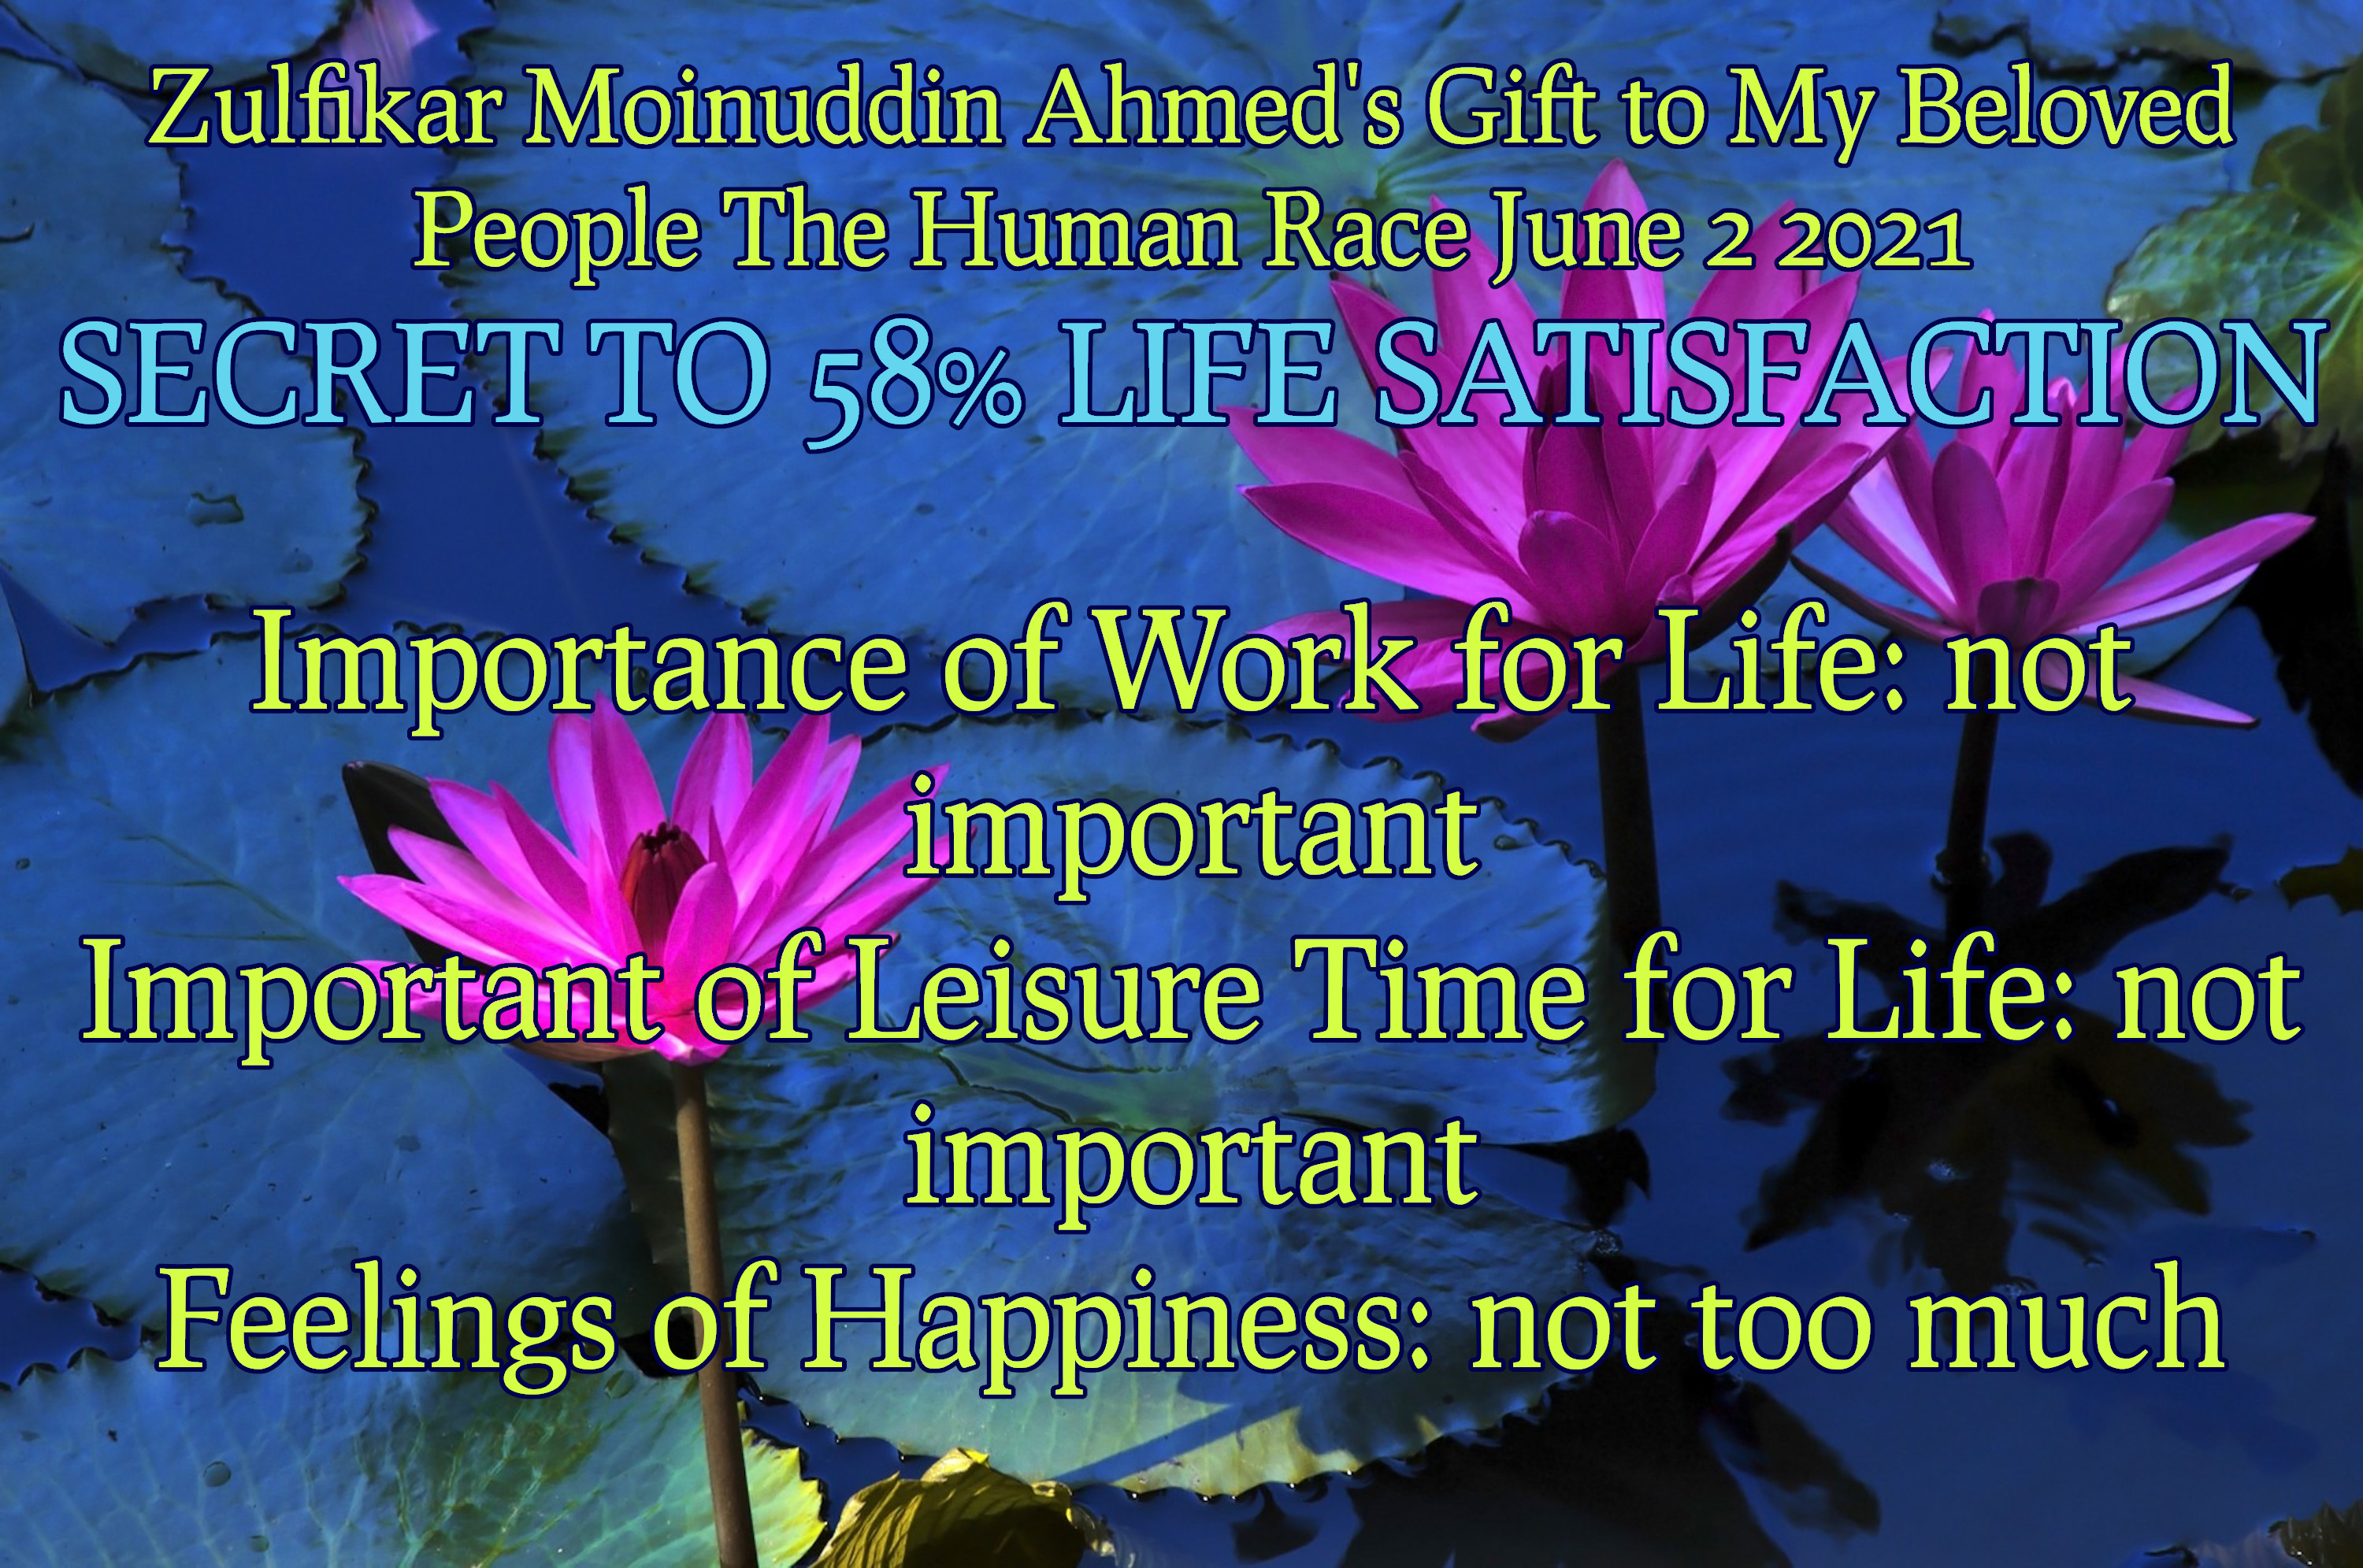
\includegraphics[scale=0.6]{secret.jpg}

\section{Life Satisfaction is Skewed To Left Politically}

The effect is subtle.

\begin{verbatim}
> pc<-table(na.omit(polv[,c("Q240","Q49")]))
> sum(rownrm(t(pc[,2]))[1:5])
[1] 0.5564202
> sum(rownrm(t(pc[,3]))[1:5])
[1] 0.5976744
> sum(rownrm(t(pc[,4]))[1:5])
[1] 0.5874636
> sum(rownrm(t(pc[,5]))[1:5])
[1] 0.5988406
> sum(rownrm(t(pc[,6]))[1:5])
[1] 0.5236721
> sum(rownrm(t(pc[,7]))[1:5])
[1] 0.5308292
> sum(rownrm(t(pc[,8]))[1:5])
[1] 0.5250366
> sum(rownrm(t(pc[,9]))[1:5])
[1] 0.4792004
> sum(rownrm(t(pc[,10]))[1:5])
[1] 0.4680276
\end{verbatim}

\end{document}